\documentclass{article}

% Language setting
% Replace `english' with e.g. `spanish' to change the document language
\usepackage[UTF8]{ctex}

% Set page size and margins
% Replace `letterpaper' with `a4paper' for UK/EU standard size
\usepackage[letterpaper,top=2cm,bottom=2cm,left=3cm,right=3cm,marginparwidth=1.75cm]{geometry}

% Useful packages
\usepackage{amsmath}
\usepackage{graphicx}
\usepackage[colorlinks=true, allcolors=blue]{hyperref}

\title{MA206 Homework10}
\author{12110120 赵钊}
\date{}

\begin{document}
\maketitle


\section{第1题}
\subsection{a}
画图估计如下:
\begin{figure}[!h]
    \centering
    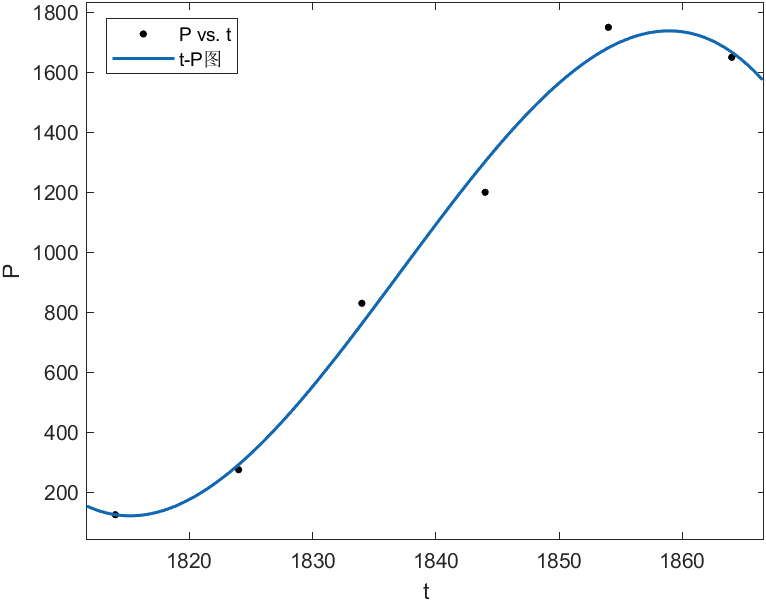
\includegraphics[width=0.75\textwidth]{pic/hw10_01.png}
    \caption{a}
\end{figure}

\subsection{b}
通过取不同的$M$值,计算$M$与$ln\left[P/(M-P)\right]$的相关系数,计算结果如下表:
\begin{table}[!ht]
    \centering
    \begin{tabular}{|l|l|l|l|l|l|l|l|}
    \hline
        M & 1900 & 1950 & 2000 & 2050 & 2100 & 2150 & 2200 \\ \hline
        Cov(t,ln[P/(M-P)]) & 0.963948 & 0.966361 & 0.967412 & 0.967758 & 0.967713 & 0.967439 & 0.967032 \\ \hline
    \end{tabular}
\end{table}

\newpage

发现$M = 2050$时,相关性最大,此时的数据如下表:

\begin{table}[!ht]
    \centering
    \begin{tabular}{|l|l|l|}
    \hline
        t & P & ln[P/(M-P)] \\ \hline
        1814 & 125 & -2.734367509 \\ \hline
        1824 & 275 & -1.864784604 \\ \hline
        1834 & 830 & -0.385180437 \\ \hline
        1844 & 1200 & 0.344840486 \\ \hline
        1854 & 1750 & 1.763588592 \\ \hline
        1864 & 1650 & 1.41706602 \\ \hline
    \end{tabular}
\end{table}

拟合得到:
\[ln\left[P/(2050-P)\right] = 0.0925t - 170.3\]

即
\[P(t) = \frac{2050}{e^{-0.0925t+170.3}+1}\]


\section{第2题}
\subsection{a}
2个主要影响:
\begin{enumerate}
    \item 微分方程中的参数$k$会影响方程的变化率,从而影响峰值的大小。
    \item 参数$N$影响取到极大或极小值的时候,自变量$X$的值。
\end{enumerate}

\subsection{b}
以$k = 1$,$N = 4$为例:
\begin{figure}[!h]
    \centering
    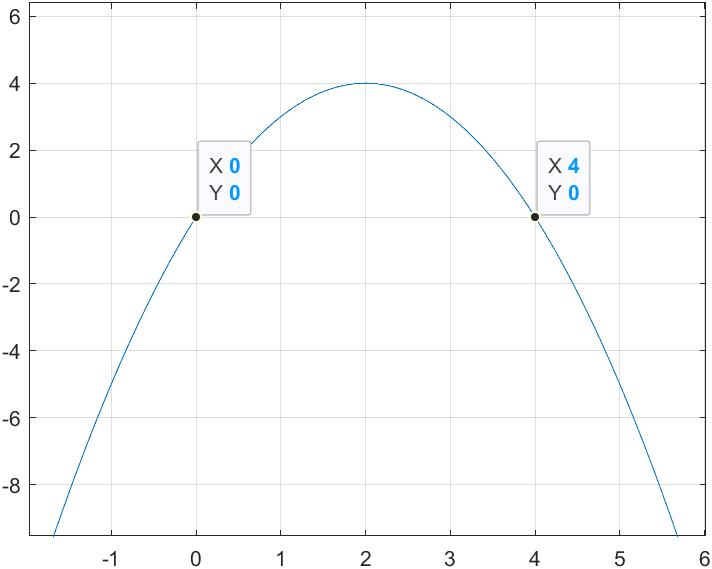
\includegraphics[width=0.6\textwidth]{pic/hw10_02.png}
    \caption{b}
\end{figure}

\subsection{c}
$X_1 < N / 2$:
\begin{figure}[!h]
    \centering
    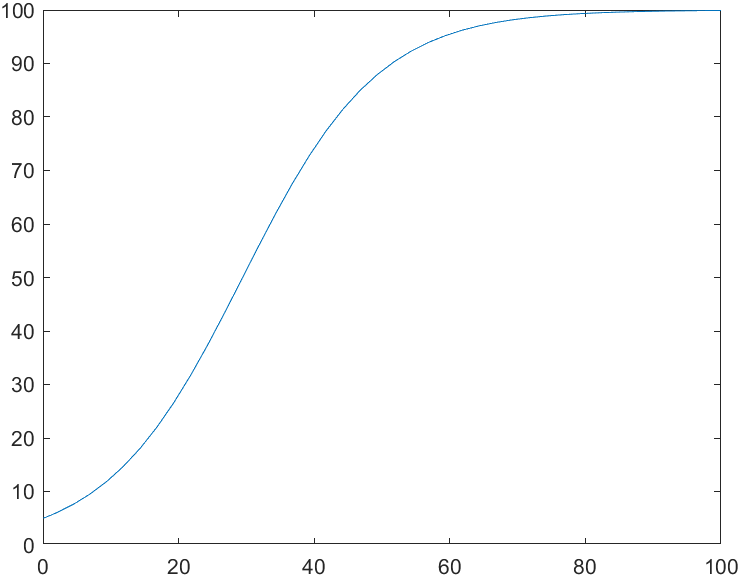
\includegraphics[width=0.6\textwidth]{pic/hw10_04.png}
    \caption{c-1}
\end{figure}

$X_2 > N / 2$:
\begin{figure}[!h]
    \centering
    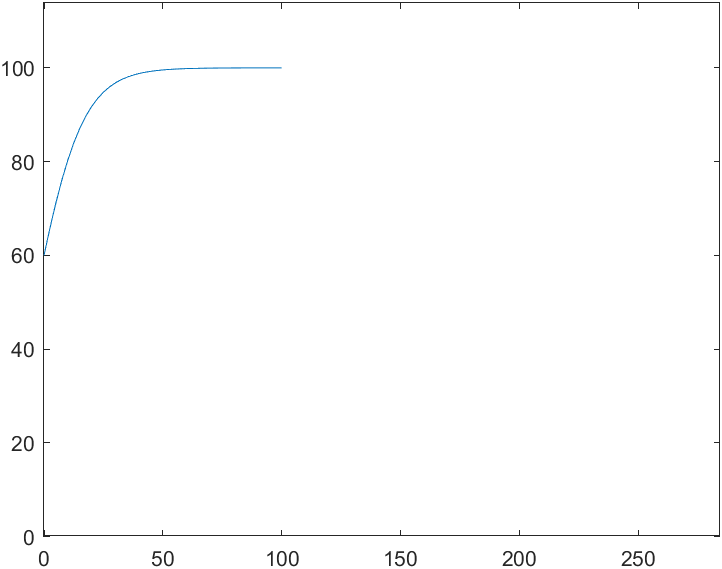
\includegraphics[width=0.6\textwidth]{pic/hw10_03.png}
    \caption{c-2}
\end{figure}

\newpage

\subsection{d}
原微分方程可变性为
\[\frac{dX}{X(N-X)} = kdt\]
对两边进行积分可得
\[\int \frac{1}{N}\left( \frac{1}{X} + \frac{1}{N-X} \right)dX = \int kdt\]
计算可得
\[\frac{1}{N} ln\frac{X}{N-X} = kt\]
\[\frac{X}{N-X} = e^{kNt}\]
\[\frac{N}{X} = e^{-kNt} + 1\]
那么有
\[X(t) = \frac{N}{e^{-kNt} + 1}\]

\subsection{e}
因为$k>0$、$N>0$,因此当$t \rightarrow \infty$时,$e^{-kNt}\rightarrow0 $,所以$X \rightarrow N$


\end{document}
